\documentclass{article}

\usepackage{xcolor, graphicx}
\usepackage{hyperref}
\usepackage{xepersian}
\settextfont{B Nazanin}
\defpersianfont\Arial{Arial}
\title{سامانه مدیریت دانش آموز}
\author{
	امیررضا سهرابی چیرانی\\
	رایان سعیدی کیا
}
\begin{document}
	\maketitle
	\cleardoublepage
	\section*{{\huge \textcolor{red}{\textbf{توضیحات}}}}
	\subsection*{این برنامه چیست؟}
	
	این برنامه طراحی شده است تا به مدیران و معاونان مدرسه دبستان و دبیرستان کمک کند.در این برنامه شما میتوانید \textbf{نام و نام خانوادگی، نمره نیمسال اول و نیمسال دوم، نام و شعبه کلاس} را وارد کنید.
	
	\subsection*{این برنامه چگونه کار میکند؟}
	این برنامه توسط زبان برنامه نویسی پایتون $ (Python) $ و فریم ورک\footnote{\Arial{framework}} پای کیو تی $ (PyQt) $ تشکیل شده است و برای ذخیره اطلاعات از دیتابیس\footnote{\Arial{database}} اس کیو ال لایت $ (SQLite) $ استفاده شده است.
	
	\begin{figure}[h!]
		\centering
		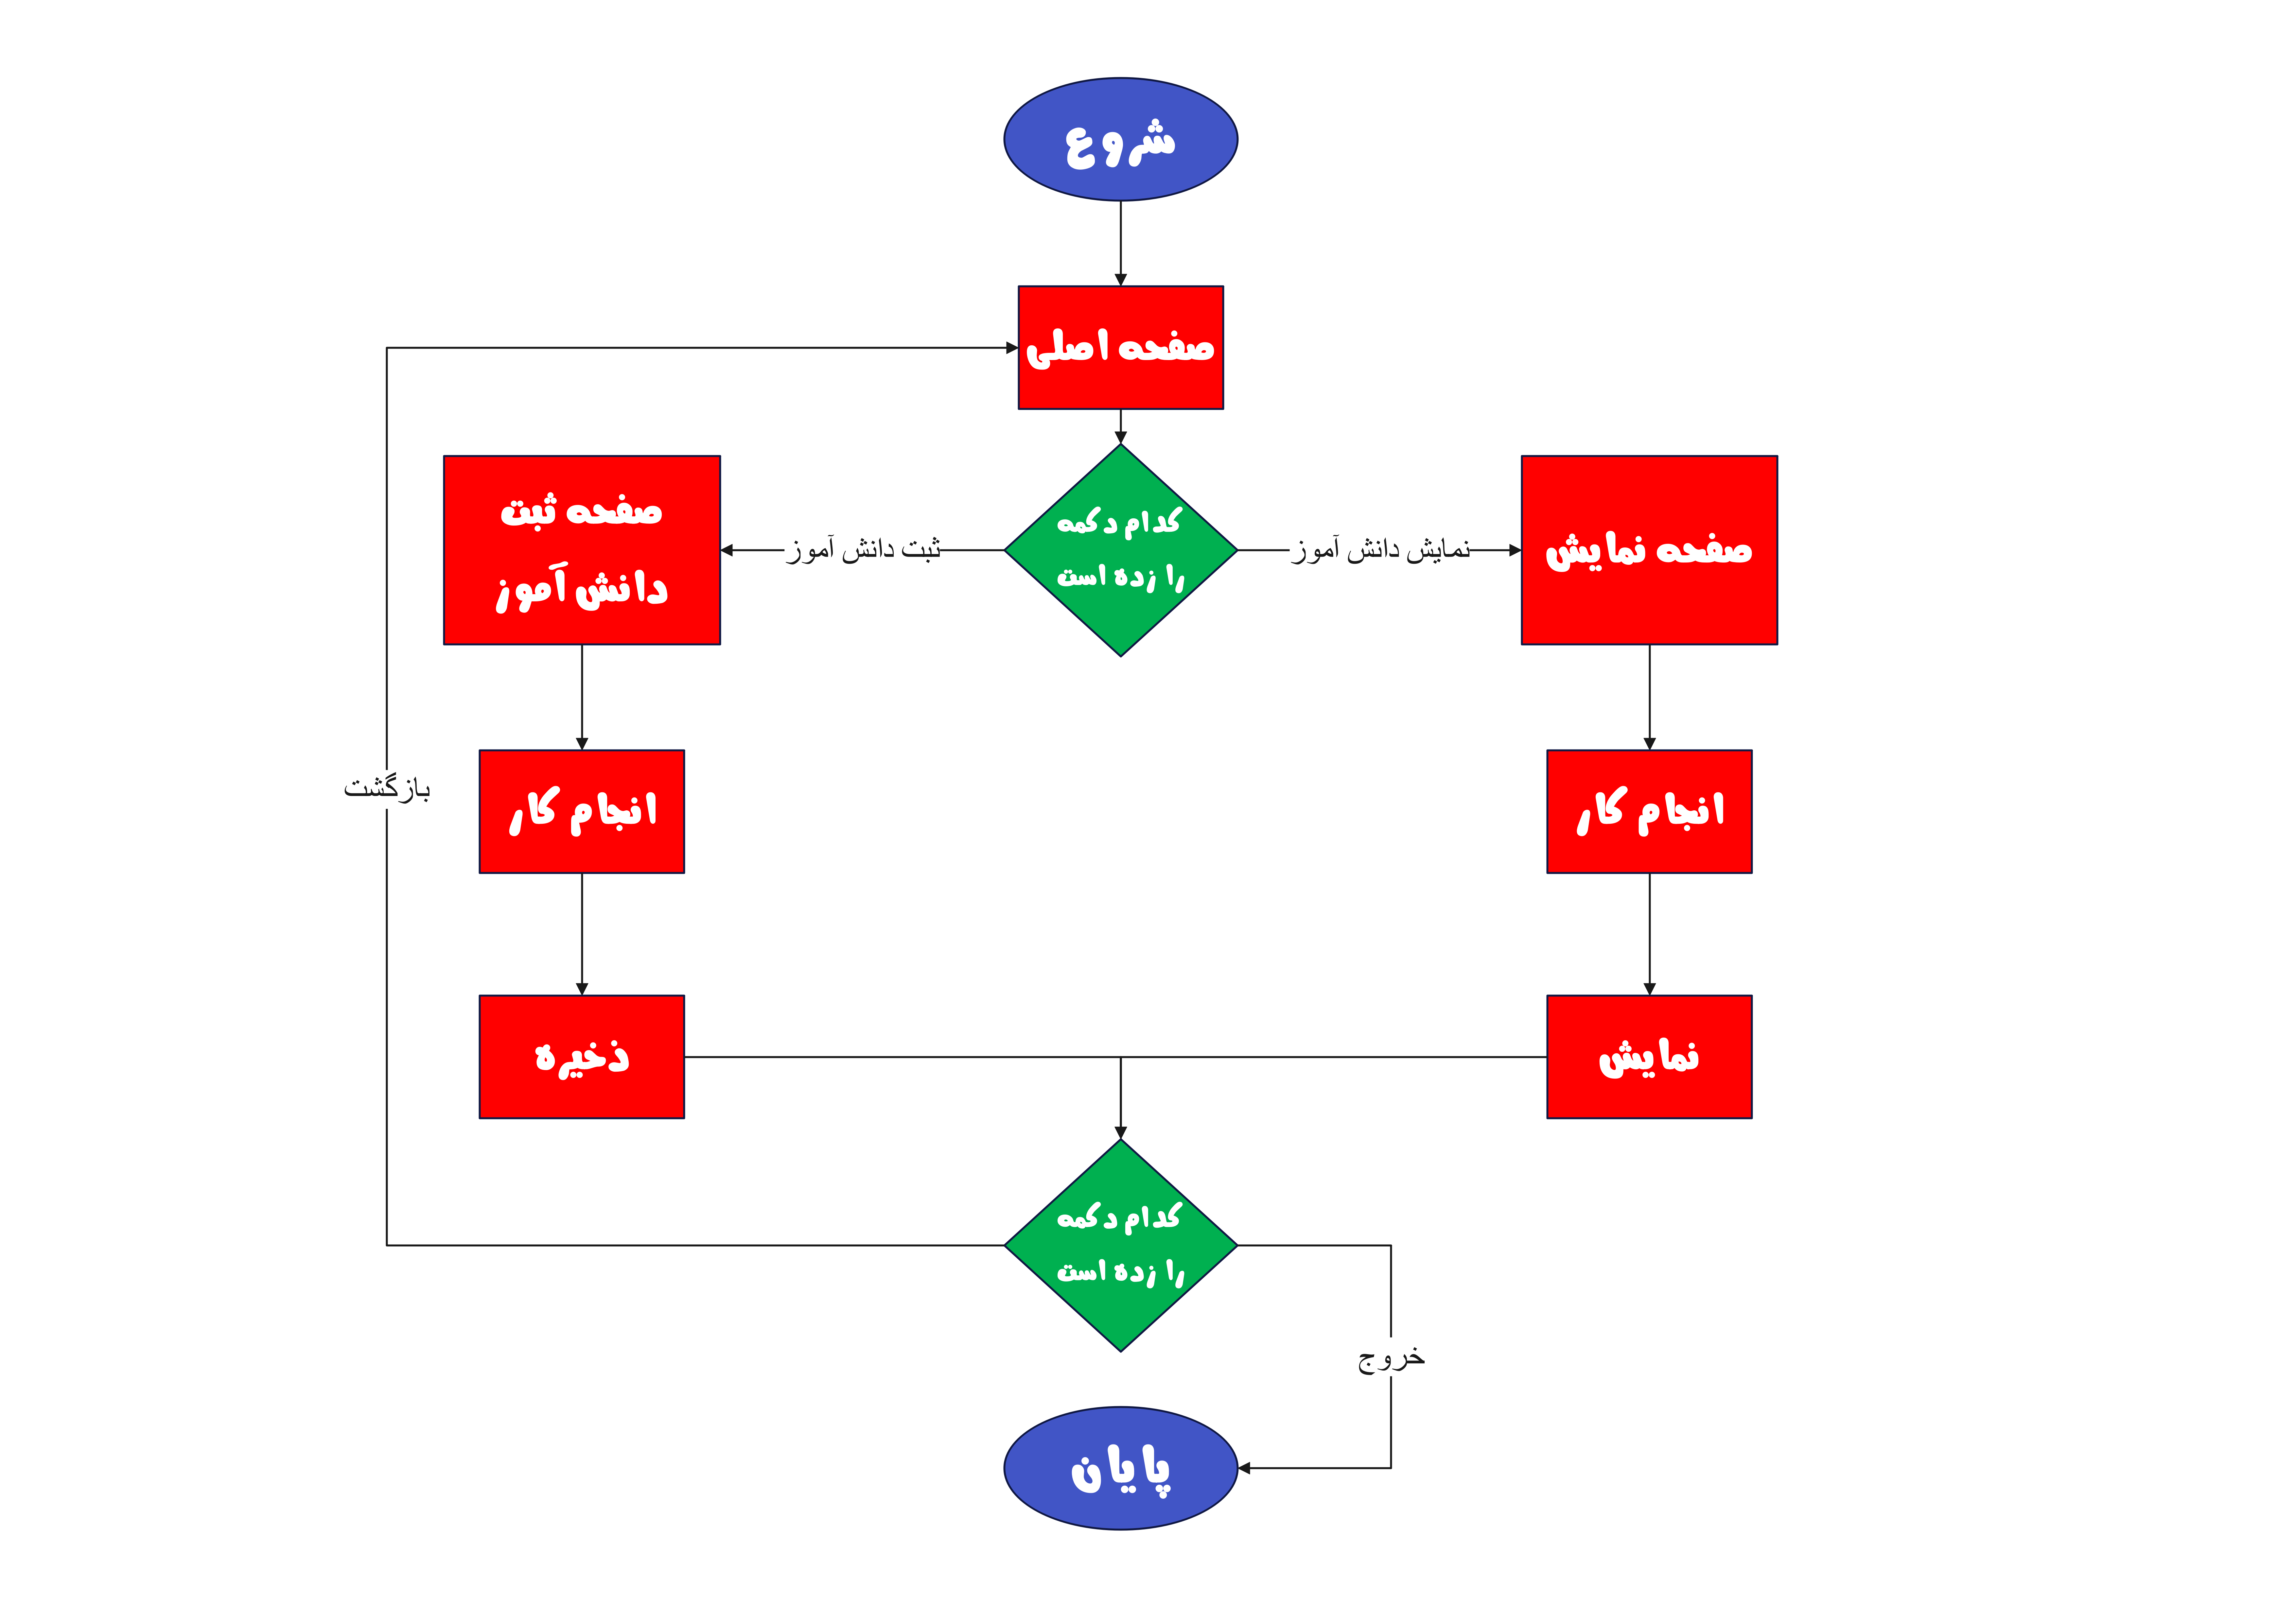
\includegraphics[width=\linewidth]{flo.png}
		\caption{فلوچارت برنامه}\label{pic1}
	\end{figure}

همانطور که در شکل \ref{pic1} دیدید برنامه از سه صفحه اصلی تشکیل شده است و در هر صفحه اجزایی برای ورودی و خروجی قرار دارد.\\

\begin{center}
	{\LARGE\textbf{ ممنون که از ما حمایت میکنید!}}
\end{center}
\cleardoublepage
\begin{latin}
\section*{{\huge \textcolor{red}{\textbf{explanations}}}}
\subsection*{What is this program?}
This program is designed to help principals and assistant principals of elementary and high schools. In this program, you can
Enter the name and family name, first semester and second semester grades, class name and branch.

\subsection*{How does this program work?}
This program is made by Python programming language and PyQt framework.
SQLite database is used to store information.

\begin{figure}[h!]
	\centering
	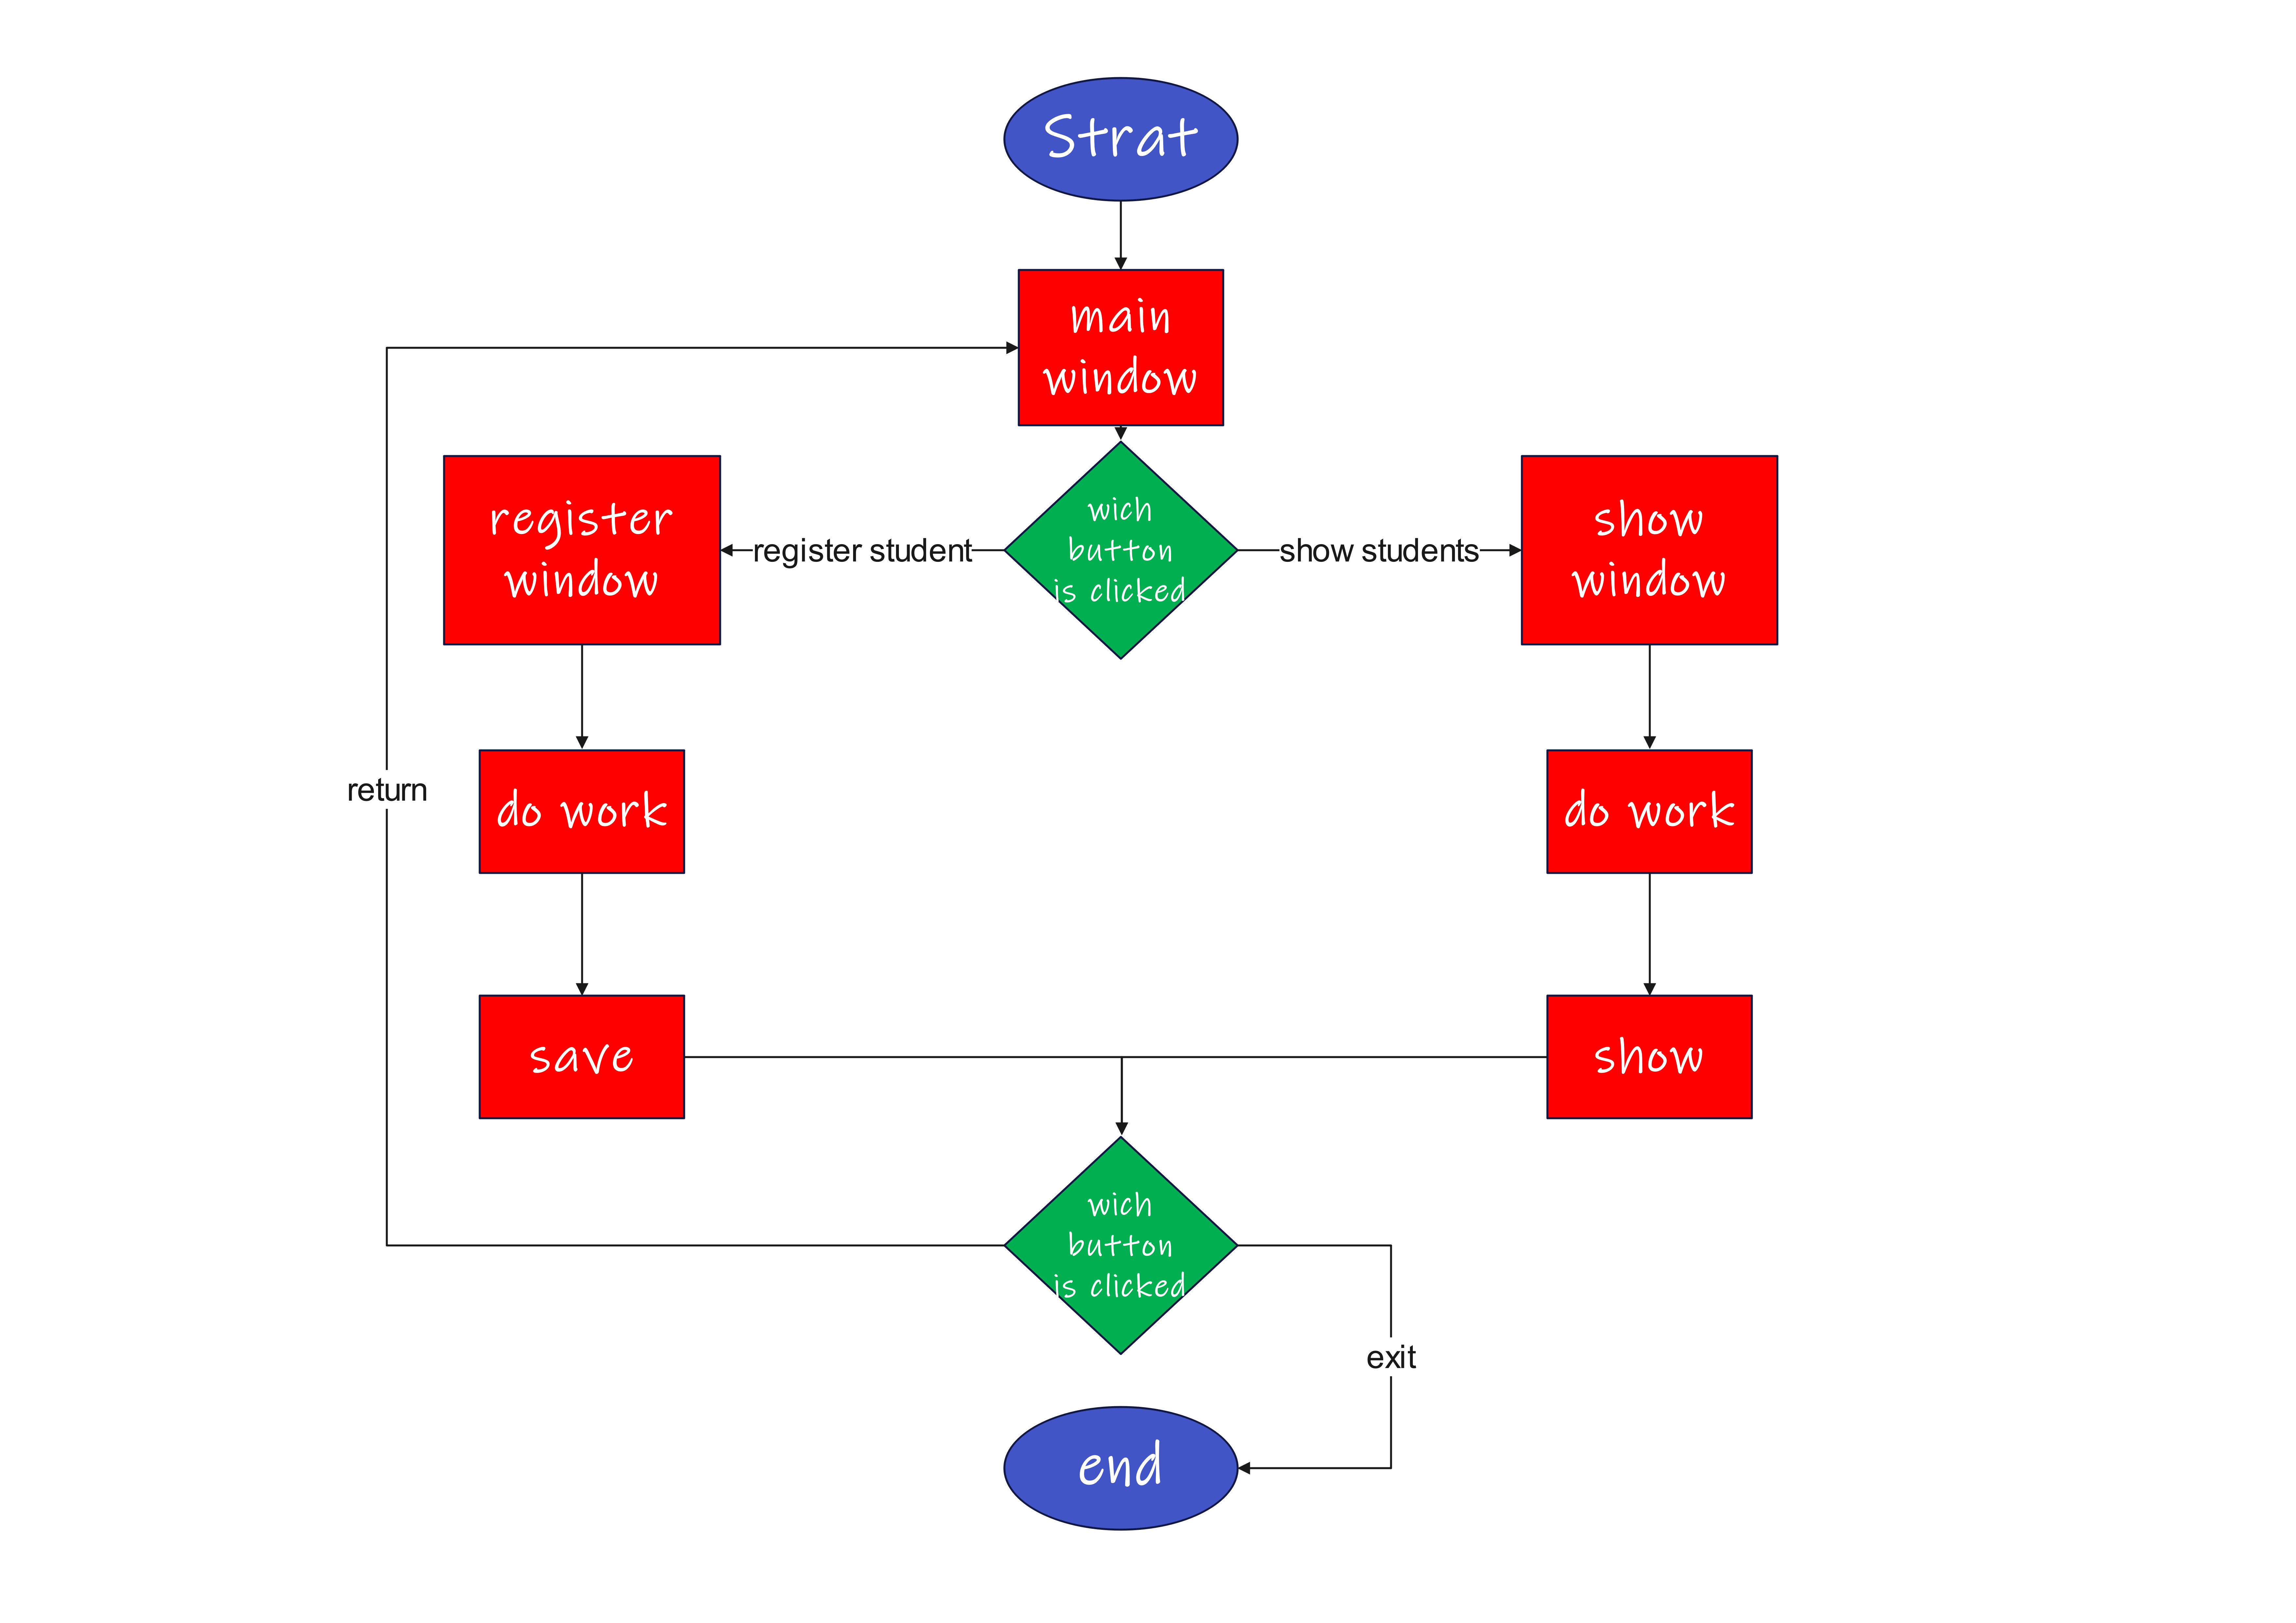
\includegraphics[width=\linewidth]{floen.png}
	\caption{flowchart of program}\label{pic2}
\end{figure}

The program you saw in Figure \ref{pic2} is described from three main pages, and each page contains components for entering.
And there is an exit.\\
\begin{center}
{\LARGE\textbf{ Thank you for supporting us!}}
\end{center}
\end{latin}
\end{document}